%
% c02-separation.tex
%
% (c) 2008 Prof Dr Andreas Mueller
% $Id: c02-separation.tex,v 1.3 2008/09/13 23:01:45 afm Exp $
%
\lhead{Separation der Variablen}
\rhead{}
\chapter{Separation der Variablen\label{chapter-separation}}
\index{Stroboskop}
\index{Eigenschwingung}
\index{stehende Welle}
\begin{figure}
\begin{center}
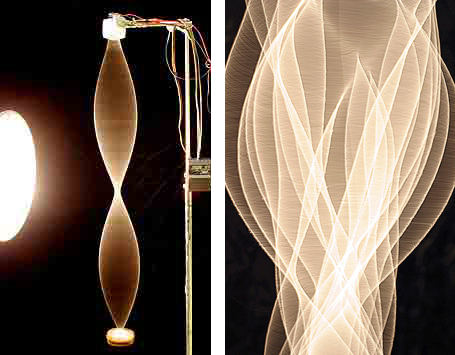
\includegraphics[width=0.8\hsize]{graphics/stringvibrlarge-10-06-06.jpg}
\end{center}
\caption{Schwingende Saite (Bild von A.~Davidhazy, http://people.rit.edu/andpph/)
\label{separation:schwingendesaite}}
\end{figure}
Beleuchtet man eine schwingende Saite mit einem Stroboskop mit der
Frequenz der Eigenschwingung, scheint die Saite stillzustehen. 
In periodischen Zeit\-ab\-st"an\-den sieht die L"osung der Wellengleichung
also gleich aus.
Misst man andererseits die Auslenkung der Saite
an einer Stelle in Abh"angigkeit von der Zeit, beobachtet man
eine harmonische Schwingung, die sich mit Hilfe von $\sin$- und
$\cos$-Funktionen beschreiben l"asst. Man kann also vermuten,
dass die L"osung der Wellengleichung der schwingenden Saite
ein Produkt
\[
u(x,t)=X(x)\cdot\sin\omega t\quad\text{oder}\quad X(x)\cdot\cos\omega t.
\]
ist. Ziel dieses Kapitels ist, diese Idee zu einem L"osungsverfahren
weiterzuentwickeln und auf einige Differentialgleichungen anzuwenden.

\section{Separation der Variablen f"ur gew"ohnliche Differentialgleichungen}
Die Differentialgleichung 
\begin{equation}
y'-xy=0
\label{separation:ode}
\end{equation}
kann mit Separation der Variablen gel"ost werden:
\begin{align*}
\frac{dy}{dx}&=xy\\
\frac1y\,dy&=x\,dx\\
\int\frac1y\,dy&=\int x\,dx\\
\log|y|&=\frac12x^2+C\\
y&=y_0e^{\frac12x^2}
\end{align*}
Das Verfahren beruht auf der Prinzip, auf jeder Seite der Gleichung
nur eine Variable zu haben.
Dabei zerlegt man sogar die Ableitung $dy/dx$, was man ja eigentlich
gar nicht darf.
Die Separation f"uhrt die L"osung der Differentialgleichung auf die
Berechnung zweier Integrale zur"uck, also eigentlich auf die
L"osung einer besonders einfachen Differentialgleichung der Form $y'=f(x)$
mit L"osung $y(x)=\int f(x)\,dx$.
Diese Form der L"osung sagt uns auch genau, was wir an Anfangsbedingungen
brauchen.
Ist $y_0$ der Wert der L"osung an der Stelle $x_0$, dann liefert
das Integral die L"osungsfunktion
\[
y(x)=\int_{x_0}^xf(\xi)\,d\xi + y_0.
\]

So einfach wird es f"ur partielle Differentialgleichungen nicht sein.
Insbesondere f"ur die an sich schon etwas ``anr"uchige'' Operationen,
den Differentialquotienten $dy/dx$ auseinanderzureissen gibt es keinerlei
Entsprechung bei partiellen Ableitungen.
Unter geeigneten Voraussetzungen an das Gebiet und die Differentialgleichung
ist es aber immer noch denkbar, dass man die Variablen trennen kann,
also 
\[
\text{Funktionen/Ableitungen nur mit $x$} = \text{Funktionen/Ableitungen nur mit $y$}
\]
Da die linke Seite nur von $x$ abh"angt, die rechte aber nur von $y$, m"ussen
beide Seiten konstant sein, die partielle Differentialgleichung zerf"allt
in eine linke {\em gew"ohnliche} Differentialgleichung f"ur eine Funktion von
$x$ und eine rechte {\em gew"ohnliche} Differentialgleichung f"ur $y$.

Da wir "uber gew"ohnliche Differntialgleichungen Bescheid wissen, sollte
es uns so m"oglich sein, eine partielle Differentialgleichung zu l"osen
und herzuleiten, welche Art von Randwerten vorgegeben werden m"ussen, damit
die Differentialgleichung eindeutig l"osbar ist.

\section{Idee des Verfahrens}
Oft hat man aus dem Anwendungsgebiet, aus dem eine partielle
Differentialgleichung stammt, Hinweise darauf, wie die L"osungsfunktion
von {\em einer} der unabh"angigen Variablen abh"angt.
Dann kann man Versuchen, die L"osung als Produkt oder Summe von
solchen ``vermuteten'' Funktionen darzustellen.

\index{Ansatz}
\index{Separationsansatz}
Aber selbst wenn man nichts "uber die L"osung weiss, kann man 
versuchen, die L"osung als Summe oder Produkt von Funktionen darzustellen,
die nur von jeweils einer Variablen abh"angen. Als Beispiel versuchen
wir die lineare Differentialgleichung 
\begin{equation}
\frac1x
\frac{\partial u}{\partial x}
+
\frac1y
\frac{\partial u}{\partial y}
=\frac1{y^2}
,
\qquad x>1, y>1
\label{separation:beispiel1}
\end{equation}
zu l"osen, wobei wir die Randbedingungen f"ur den Moment ignorieren.
Wir versuchen, die L"osung als Summe von zwei Funktionen darzustellen,
welche nur von $x$ bzw.~$y$ abh"angen, also
\begin{equation}
u(x,y)=X(x)+Y(y)
\quad\Rightarrow\quad
\begin{cases}
\quad{\displaystyle \frac{\partial u}{\partial x}}&=X'(x)\\
\\
\quad{\displaystyle \frac{\partial u}{\partial y}}&=Y'(y)\\
\end{cases}
\label{separation:beispiel1:ansatz}
\end{equation}
Setzt man dies in die Differentialgleichung (\ref{separation:beispiel1})
ein, erhalten wir die Gleichung
\[
\frac{X'(x)}{x}+\frac{Y'(y)}{y}=\frac1{y^2}
\]
der
\begin{equation}
\frac{X'(x)}{x}
=\frac1{y^2}
-\frac{Y'(y)}{y}.
\label{separation:beispiel1:separiert}
\end{equation}
Die Form (\ref{separation:beispiel1:separiert}) hat eine besondere
Eigenschaft: die Variable $x$ kommt nur auf der linken Seite vor,
die Variable $y$ nur auf der rechten. Setzt man f"ur $y$ irgend
einen Wert ein, ver"andert sich die rechte Seite nicht mehr,
die linke Seite muss also f"ur alle $x$ den gleichen Wert geben.
L"asst man jetzt wieder das $y$ varieren, muss sich auch auf der rechten
Seite immer der gleiche Wert geben. Wir nennen den gemeinsamen Wert
$k$, und bekommen zwei gew"ohnliche Differentialgleichungen
f"ur $X(x)$ und $Y(y)$:
\begin{align}
\frac{X'(x)}{x}&=k
&
k&=\frac1{y^2}-\frac{Y'(y)}{y}
\label{separation:beispiel1:separiertedgl}
\end{align}
Die linke Differentialgleichung ist einfach zu l"osen:
\begin{align*}
X'(x)&=kx\quad\Rightarrow\quad X(x)=
\frac12kx^2+C_x.
\end{align*}
Die rechte Differentialgleichung ist nur leicht komplizierter:
\begin{align*}
Y'(y)=\frac1y-ky
\quad\Rightarrow\quad
Y(y)=\int\frac1y-ky\,dy=
\log y-\frac12ky^2+C_y.
\end{align*}
Diese beiden L"osungen k"onnen wir jetzt wieder zu einer L"osung der
urspr"unglichen Differentialgleichung zusammensetzen:
\begin{equation}
u(x,y)=
\frac12kx^2+
\log y-\frac12ky^2+C.
\label{separation:beispiel1:loesung}
\end{equation}
Wir haben damit eine unendliche Familie von L"osungen der
Differentialgleichung gefunden, f"ur jedes Paar $(k,C)$ von
Parametern liefert die Formel (\ref{separation:beispiel1:loesung})
eine L"osung.
Dazu m"ussen wir in irgend einer Weise die Randbedingungen verwenden.
Damit haben wir eine Skizze f"ur das L"osungsverfahren mit Separation:
\begin{enumerate}
\item Finde einen L"osungsansatz aus Funktionen, die nur von einer
Variablen abh"angen.
\item Setze in die Differentialgleichung ein und separiere die Terme
so, dass zwei Variablen jeweils nur auf einer Seite vorkommen. Dann
h"angen beide Seiten nicht mehr von dieser Variablen ab, jede Seite
ist eine Differentialgleichung mit weniger Variablen.
\item L"ose die Teildifferentialgleichungen, und setze daraus 
L"osungen zusammen. 
\item Verwende die Randbedingungen, um eine L"osung zu finden.
\end{enumerate}
Wie man unschwer erkennen kann, ist weniger die L"osung der
einzelnen Teildifferentialgleichungen das Problem, sondern der letzte
Schritt. In den folgenden Abschnitten zeigen wir an Beispielen, wie
dies m"oglich ist.

\section{Separation f"ur lineare partielle Differentialgleichungen}
Die Grundidee des Seoparationsverfahrens liefert eine Familie von Funktionen,
von ein paar Integrationskonstanten abh"angen. Vorgegeben sind auf dem
Rand aber beliebige Funktionen, es ist im Allgemeinen nicht m"oglich,
durch richtige Wahl von wenigen Parametern beliebige Funktionen zu erhalten.
Des Separationsverfahren in der bisherigen Form kann also ein
beliebiges Randwertproblem noch nicht l"osen.

Nehmen wir an, es m"usse die Differentialgleichung $Lu=f$ auf dem
Gebiet $\Omega$ mit Randwerte $g(x)$ f"ur $x\in\partial \Omega$
gel"ost werden.
Wir haben nur dann eine Chance, aus den bisherigen Resultaten eine 
vollst"andige L"osung des Problems zu erhalten, wenn wir in der
Lage sind, solche Teill"osungen zu einer vollst"andigen L"osung
zu kombinieren. Dazu sind aber im allgemeinen zus"atzliche
Bedingungen an die Differentialgleichung n"otig. Linearit"at der
Differentialgleichung ist, was wir hier verwenden wollen:

\begin{satz}Sind $u_1$ und $u_2$ L"osungen einer homogenen linearen partiellen
Differentialgleichung, dann sind auch $u_1+u_2$ und $\lambda u_1$ f"ur
$\lambda\in\mathbb R$ L"osungen
\end{satz}

\begin{proof}[Beweis]
Die Differentialgleichung
\[
F(x_1,\dots,x_2,u,\frac{\partial u}{\partial x_1},\dots)=0
\]
ist linear in $u$ und den Ableitungen, man darf also Summen und Vielfache
in $u$ und den Ableitungen aus der Funktion herausziehen:
\begin{align*}
F(x_1,\dots,x_2,u_1+u_2,\frac{\partial u_1}{\partial x_1}+\frac{\partial u_2}{\partial x_1},\dots)
&=
F(x_1,\dots,x_2,u_1,\frac{\partial u_1}{\partial x_1},\dots)
\\
&+
F(x_1,\dots,x_2,u_2,\frac{\partial u_2}{\partial x_1},\dots)=0
\\
F(x_1,\dots,x_2,\lambda u_1,\frac{\partial \lambda u_1}{\partial x_1},\dots)
&=
\lambda
F(x_1,\dots,x_2,u_1,\frac{\partial u_1}{\partial x_1},\dots)
=0
\end{align*}
Die Linearkombinationen von $u_1$ und $u_2$ sind also auch L"osungen.
\end{proof}

Um die Differentialgleichung zu l"osen, kann man also versuchen, mit
dem bisherigen Separationsverfahren m"oglichst viele L"osungen zu
$u_1$, $u_2$, $u_3,\dots$ zu finden, und diese dann zu einer Gesamtl"osung
zu kombinieren
\[
u(x)=\sum_{i=1}^\infty a_ku_k
\]
mit geeigneten Koeffizienten $a_k$, die so zu w"ahlen sind, dass die
Randbedingungen erf"ullt sind.

Inhomogene lineare partielle Differentialgleichungen k"ann man mit diesem
Verfahren ebenfalls l"osen. Dazu findet man zun"achst eine partikul"are
L"osung $u_p$, welche die inhomogenen Differentialgleichung l"ost, ohne
allerdings korrekte Randwerte zu liefern.
Das urspr"ungliche Separationsverfahren kann hierbei hilfreich sein.
Dann verwendet man das skizzierte Verfahren f"ur homogene lineare
partielle Differentialgleichungen f"ur modifizierte Randwerte $g-u_p$ auf
$\partial\Omega$ um eine L"osung der homogenen Gleichung $u_h$ zu finden.
Die Summe $u=u_p+u_h$ ist dann eine L"osung der inhomogenen Gleichung
mit Randwerten $u_p + (g-u_p)=g$, also ein L"osung des urspr"unglichen
Problems.

Die Bestimmung der Koeffizienten $a_k$ f"ur die gefundene Familie
von Teill"osungen f"uhrt oft auf die Fourier-Theorie, oder allgemeiner
auf orthogonale Funktionenfamilien. Solche Teill"osungen haben oft eine
unmittelbare physikalische Bedeutung, zum Beispiel treten sie auf als
Schingungsmoden (in der Mechanik oder Elektrotechnik) oder als
Elektronenzust"ande in der Quantenmechanik.

\section{Schwingende rechteckige Membran}
\rhead{Rechteckige Membran}
\index{Membran!rechteckig}
Wir betrachten die Schwingung einer rechteckigen Membran, die am Rande
des Gebietes
\[
R=\{(x,y)\,|\,0\le x\le a,0\le y\le b\} =(0,a)\times(0,b)
\]
eingespannt ist. Zur Zeit $t=0$ sei die Form der Membran durch die
Funktion $f(x,y)$ gegeben.
F"ur beliebige Zeit $t\ge 0$ wird sie beschrieben durch eine Funktion $u(x,y,t)$,
welche der Differentialgleichung
\[
\frac1{c^2}\frac{\partial^2u}{\partial t^2}=\frac{\partial^2u}{\partial x^2}+\frac{\partial^2u}{\partial y^2}
\]
gen"ugt mit den Anfangsbedingungen
\begin{align*}
u(x,y,0)&=f(x,y)\quad\forall 0\le x\le a,0\le y\le b,
\\
\frac{\partial}{\partial t}u(x,y,0)&=g(x,y)\quad\forall 0\le x\le a,0\le y\le b
\end{align*}
und den Randbedingungen
\begin{align*}
u(0,y,t)&=0&u(a,y,t)&=0&\forall t\ge 0,0\le y\le b,\\
u(x,0,t)&=0&u(x,b,t)&=0&\forall t\ge 0,0\le x\le a.
\end{align*}

\subsection{Separation der Zeit}
\index{Separation}
Nach der in der Einleitung motivierten Idee suchen wir L"osungen also
Produkt einer Funktion $T(t)$, die nur von der Zeit abh"angt, und einer Funktion
$\varphi(x,y)$, welche nur vom Ort abh"angt, also
\[
u(x,y,t)=T(t)\cdot\varphi(x,y).
\]
Leider kann ein einzelnes solches Produkt nicht alle Anfangsbedingungen
erf"ullen. W"are dies n"amlich m"oglich, m"usste $\varphi(x,y)\sim f(x,y)$
sein und alle Teile der Membran w"urden im Gleichtakt hin und her schwingen.
Simulationen oder physikalische Experimente zeigen aber, dass es
Anfangsbedingungen gibt, bei denen die Teile der Membran gegenl"aufig
schwingen.

Anderseits, muss die L"osung auf jeden Fall die Randbedingung erf"ullen,
es muss also gelten
\begin{align*}
\varphi(0,y)&=0&\varphi(a,y)&=0&0\le y\le b\\
\varphi(x,0)&=0&\varphi(x,b)&=0&0\le x\le a
\end{align*}
Setzen wir diesen Ansatz f"ur $u$ in der Wellengleichung ein,
erhalten wir
\[
\frac1{c^2}T''(t)\varphi(x,y)=T(t)\left(
\frac{\partial^2\varphi}{\partial x^2}
+
\frac{\partial^2\varphi}{\partial y^2}
\right)
\]
Wir suchen eine Funktion $u$, die nicht identisch verschwindet,
es gibt also einige Zeitpunkte $t$ und Orte $(x,y)$, an denen $T(t)$
und $\varphi(x,y)$ nicht verschwinden. An diesen Stellen kann man die
Gleichung umformen in
\begin{equation}
\frac1{c^2}\frac{T''(t)}{T(t)}
= \frac1{\varphi(x,y)}\left( \frac{\partial^2\varphi}{\partial x^2}
+ \frac{\partial^2\varphi}{\partial y^2} \right)
\label{separiert}
\end{equation}
Die rechte Seite h"angt nur
vom Ort ab, darf sich also nicht "andern, wenn man die Zeit $t$ variert.
Als Funktion der Zeit muss die linke Seite eine Konstante sein,
es gibt also ein $k$ mit der Eigenschaft
\[
\frac1{c^2}\frac{T''(t)}{T(t)}=k
\qquad\Leftrightarrow\qquad
T''(t)=k T(t).
\]
Diese gew"ohnliche Differentialgleichung hat L"osungen der Form 
$e^{\pm\sqrt{k}t}$ f"ur positives $k$. F"ur negatives $k$ sind $\sin\sqrt{k}t$ 
und $\cos\sqrt{k}t$ L"osungen.
Aus physikalischer Sicht sind nur L"osungen mit Schwingungscharakter sinnvoll,
wir k"onnen daher annehmen, dass $k<0$.
Ein solches $k$ l"asst sich in der Form $k=-\lambda^2$ schreiben.
Es gibt also ein $\lambda$ mit der Eigenschaft
\[
\frac1{c^2}\frac{T''(t)}{T(t)}=-\lambda^2
\]
oder
\[
T''(t)=-c^2\lambda^2 T(t).
\]
Dies ist eine gew"ohnliche Differentialgleichung zweiter Ordnung, welche mit
bekannten Methoden gel"ost werden kann.
Die allgemeine L"osung dieser Gleichung ist von der Form
\[
A\cos c\lambda t+B\sin c\lambda t.
\]

\subsection{Reduktion auf ein Eigenwertproblem}
\index{Eigenwertproblem}
Die linke Seite von (\ref{separiert}) h"angt nur von der Zeit ab, darf sich
also nicht "andern, wenn man $x$ oder $y$ variert. Als Funktion des Ortes
muss die rechte Seite also ebenfalls konstant sein:
\begin{align*}
\frac1{\varphi(x,y)}\left(
\frac{\partial^2\varphi}{\partial x^2}
+
\frac{\partial^2\varphi}{\partial y^2}
\right)&=-\lambda^2\\
\frac{\partial^2\varphi}{\partial x^2}
+
\frac{\partial^2\varphi}{\partial y^2}
=\Delta\varphi
&=-\lambda^2
\varphi(x,y)
\end{align*}
Die gesuchte Funktion $\varphi$ ist also ein Eigenvektor des linearen
Operators $\Delta$ zum Eigenwert $-\lambda^2$.
Nur die Eigenwerte des Operator $\Delta$ kommen also f"ur die
Zeitabh"angigkeitsgleichung in Frage.

\subsection{Separation von $x$ und $y$}
\index{Separation}
F"ur das Eigenwertproblem k"onnen wir erneut den Separationsansatz
\[
\varphi(x,y)=X(x)\cdot Y(y)
\]
versuchen.
Einsetzen in die Differentialgleichung ergibt
\begin{align*}
X''(x)Y(x)+X(x)Y''(y)&=-\lambda^2 X(x)Y(y)
\\
\frac{X''(x)}{X(x)}+\frac{Y''(y)}{Y(y)}&=-\lambda^2
\end{align*}
Jeder der Br"uche h"angt nur von jeweils einer Variable ab, was nur
m"oglich ist, wenn beide Terme konstant sind. Damit ist das Problem
reduziert auf zwei Gleichungen
\begin{align*}
X''(x)&=-\lambda_1^2X(x)\\
Y''(y)&=-\lambda_2^2Y(y)\\
\lambda_1^2+\lambda_2^2&=\lambda^2
\end{align*}
Die allgemeinen L"osungen dieser Gleichungen, die auch die Randbedingung
bei $x=0$ bzw.~$y=0$ erf"ullt, sind
\begin{align*}
X(x)&=A\sin \lambda_1x\\
Y(y)&=B\sin \lambda_2y
\end{align*}
Die Randbedingungen f"ur $x=a$ und $y=b$ k"onnen nur erf"ullt werden,
wenn $\lambda_1a$ und $\lambda_2b$ Vielfache von $\pi$ sind, also
\[
\lambda_1=\frac{k\pi}a
\qquad
\text{und}
\qquad
\lambda_2=\frac{l\pi}b
\]
Die m"oglichen Werte von $\lambda$ sind also
\[
\lambda_{kl}^2=\left(\frac{k^2}{a^2} + \frac{l^2}{b^2}\right)\pi^2,\qquad k,l\in\mathbb Z
\]
Damit kann man jetzt die allgemeine L"osung des Schwingungsproblems aus den
Teill"osungen
\[
\varphi_{kl}(x,y)=\sin \frac{k\pi}{a}x\sin\frac{l\pi}{b}y
\]
f"ur das Eigenwertproblem
und den Teill"osungen
\[
u_{kl}(x,y,t)
=
(A_{kl}\cos c\lambda_{kl} t+
B_{kl}\sin c\lambda_{kl} t)
\sin \frac{k\pi}{a}x\sin\frac{l\pi}{b}y
\]
f"ur das zeitabh"angige Problem
zu einer allgemeinen L"osung
\begin{equation}
u(x,y,t)=\sum_{k,l}
(A_{kl}\cos c\lambda_{kl} t+
B_{kl}\sin c\lambda_{kl} t)
\sin \frac{k\pi}{a}x\sin\frac{l\pi}{b}y
\label{allgemeineloesung}
\end{equation}
zusammensetzen.

\subsection{Anfangsbedingungen}
\index{Anfangsbedingungen}
Die allgemeine L"osung muss jetzt auch noch die Anfangsbedingung erf"ullen:
\begin{align*}
\sum_{k,l}A_{kl}
\sin \frac{k\pi}{a}x\sin\frac{l\pi}{b}y&=f(x,y)\\
\sum_{k,l}B_{kl}c\lambda_{kl}
\sin \frac{k\pi}{a}x\sin\frac{l\pi}{b}y&=g(x,y)\\
\end{align*}
Die Koeffizienten $A_{kl}$ und $B_{kl}$ k"onnen in einfachen F"allen mit
Koeffizientenvergleich und im Allgemeinen mit Hilfe der Theorie
der Fourierreihen berechnet werden.
\index{Fourierreihe}

\section{Kreisgebiet}
\rhead{Kreisgebiet}
\index{Kreisgebiet}
\index{Kreisscheibe}
In diesem Abschnitt betrachten wir eine Kreisscheibe
\[
G=\{(x,y)\in\mathbb R^2|x^2+y^2 < R\}
\]
mit Radius $R$ als Definitionsbereich. Da sich dieses Gebiet durch
eine Streckung um den Faktor $\frac1R$ immer auf einen Einheitskreis
abbilden l"asst, k"onnen wir ohne Verlust an Allgemeinheit vorausetzen,
dass $R=1$ ist.

Ein Kreisgebiet tritt zum Beispiel beim Problem auf, die Schwingungen
einer kreisf"ormigen Membran zu berechnen, wie sie bei einer Kesselpauke
vorkommen. Nach den Ergebnissen des ersten Kapitels suchen wir nach einer
Funktion $u$, welche auf $G$ die Gleichung
\[
\frac1{a^2}\frac{\partial^2 u}{\partial t^2}=\frac{\partial^2 u}{\partial x^2}+\frac{\partial^2 u}{\partial y^2}
\]
erf"ullt. Wie bei der Schwingung der einer rechteckigen Platte
wird daraus mit dem Ansatz $ u(x,y,t)=u(x,y)\cdot T(t)$ ein
Eigenwertproblem:
\begin{align*}
T''(t)&=-a^2\lambda^2 T(t)\\
\Delta u(x,y)&=-\lambda^2u(x,y)
\end{align*}
Das Poissonproblem ist der Spezialfall $\lambda=0$.
\index{Poissonproblem}

\subsection{Polarkoordinaten}
\index{Polarkoordinaten}
Offenbar sind Polarkoordinaten speziell gut an das Problem angepasst, 
eine Randbedingung l"asst sich zum Beispiel durch eine Funktion beschreiben,
welche nur vom Polarwinkel abh"angt.
Eine schwingende kreisf"ormite Membran f"uhrt also auf die partielle
Differentialgleichung
\[
\frac{\partial^2u(r,\varphi)}{\partial t^2}=\Delta u(r,\varphi)
\]
mit der Randbedingung
\[
u(R,\varphi)=0,\qquad\varphi\in[0,2\pi],
\]
wobei wie oben $R$ der Radius der Membran ist.

Damit das Problem auf einem Kreisgebiet in Polarkoordinaten behandelt
werden kann,
brauchen wir einen Ausdruck f"ur $\Delta u$ in Polarkoordinaten.
\begin{align}
x&=r\cos\varphi\\
y&=r\sin\varphi
\label{polarkoordinaten}
\end{align}
Um die Ableitungen nach $x$ und $y$ durch Ableitungen $\varphi$ und $r$ zu
ersetzen, leiten wir (\ref{polarkoordinaten}) nach $x$ und $y$ ab:
\begin{align*}
1&=
\frac{\partial r}{\partial x}\cos\varphi
-r\sin\varphi \frac{\partial\varphi}{\partial x}
&
0&=
\frac{\partial r}{\partial y}\cos\varphi
-r\sin\varphi \frac{\partial\varphi}{\partial y}
\\
0&=
\frac{\partial r}{\partial x}\sin\varphi
+r\cos\varphi \frac{\partial\varphi}{\partial x}
&
1&=
\frac{\partial r}{\partial y}\sin\varphi
+r\cos\varphi \frac{\partial\varphi}{\partial y}
\end{align*}
In Matrixschreibweise ist dies
\begin{align*}
\begin{pmatrix}1\\0\end{pmatrix}
&=
\begin{pmatrix}
\cos\varphi&-\sin\varphi\\
\sin\varphi&\cos\varphi
\end{pmatrix}
\begin{pmatrix}
\frac{\partial r}{\partial x}\\
r\frac{\partial \varphi}{\partial x}
\end{pmatrix}
&
\begin{pmatrix}0\\1\end{pmatrix}
&=
\begin{pmatrix}
\cos\varphi&-\sin\varphi\\
\sin\varphi&\cos\varphi
\end{pmatrix}
\begin{pmatrix}
\frac{\partial r}{\partial y}\\
r\frac{\partial \varphi}{\partial y}
\end{pmatrix}
\end{align*}
Die $2\times2$ Matrix ist eine Drehmatrix, die Inverse findet man, indem man
$\varphi$ durch $-\varphi$ ersetzt. Die Multiplikation auf der linken Seite
ergibt jeweils die erste bzw. zweite Spalte der Drehmatrix zum
Winkel $\varphi$:
\begin{align*}
\cos\varphi
&=\frac{\partial r}{\partial x}
&&
&
\sin\varphi
&=
\frac{\partial r}{\partial y}
&&
\\
-\sin\varphi
&=r\frac{\partial \varphi}{\partial x}
&\Rightarrow\quad
\frac{\partial\varphi}{\partial x}&=-\frac1r\sin\varphi
&
\cos\varphi
&=
r\frac{\partial\varphi}{\partial y}
&\Rightarrow\quad
\frac{\partial\varphi}{\partial y}&=\frac1r\cos\varphi
\end{align*}
Mit diesen Formeln k"onnen wir jetzt die h"oheren Ableitungen
von $u$ nach  $x$ und $y$ durch Ableitungen nach $r$ und $\varphi$
ersetzen.

Die partiellen Ableitungen von $\varphi$ nach $x$ und $y$ sind
\begin{align*}
\frac{\partial u}{\partial x}
&=
\frac{\partial u}{\partial r}
\frac{\partial r}{\partial x}
+
\frac{\partial u}{\partial\varphi}
\frac{\partial \varphi}{\partial x}
=
\frac{\partial u}{\partial r}
\cos\varphi
-
\frac{\partial u}{\partial\varphi}
\frac1r\sin\varphi
\\
\frac{\partial u}{\partial y}
&=
\frac{\partial u}{\partial r}
\frac{\partial r}{\partial y}
+
\frac{\partial u}{\partial\varphi}
\frac{\partial \varphi}{\partial y}
=
\frac{\partial u}{\partial r}
\sin\varphi
+
\frac{\partial u}{\partial\varphi}
\frac1r\cos\varphi
\end{align*}
Die zweiten Ableitungen sind
\begin{align*}
\frac{\partial^2u}{\partial x^2}
&=
\frac{\partial}{\partial r}
\left(
\frac{\partial u}{\partial r}
\cos\varphi
-
\frac{\partial u}{\partial\varphi}
\frac1r\sin\varphi
\right)
\frac{\partial r}{\partial x}
+
\frac{\partial }{\partial \varphi}
\left(
\frac{\partial u}{\partial r}
\cos\varphi
-
\frac{\partial u}{\partial\varphi}
\frac1r\sin\varphi
\right)
\frac{\partial\varphi}{\partial x}
\\
&=
\frac{\partial}{\partial r}
\left(
\frac{\partial u}{\partial r}
\cos\varphi
-
\frac{\partial u}{\partial\varphi}
\frac1r\sin\varphi
\right)
\cos\varphi
-
\frac{\partial }{\partial \varphi}
\left(
\frac{\partial u}{\partial r}
\cos\varphi
-
\frac{\partial u}{\partial\varphi}
\frac1r\sin\varphi
\right)
\frac1r\sin\varphi
\\
&=
\frac{\partial^2u}{\partial r^2} \cos^2\varphi
-
\frac{\partial^2u}{\partial r\partial\varphi} \frac1r\sin\varphi \cos\varphi
+
\frac{\partial u}{\partial\varphi} \frac1{r^2}\sin\varphi\cos\varphi
\\
&\quad
-
\frac{\partial^2u}{\partial\varphi\partial r}\frac1r \cos\varphi\sin\varphi
+\frac{\partial u}{\partial r}\frac1r\sin^2\varphi
+\frac{\partial^2u}{\partial\varphi^2}
\frac1{r^2}\sin^2\varphi
+\frac{\partial u}{\partial\varphi}\frac1{r^2}\cos\varphi\sin\varphi
\\
\frac{\partial^2u}{\partial y^2}
&=
\frac{\partial}{\partial r}
\left(
\frac{\partial u}{\partial r}
\sin\varphi
+
\frac{\partial u}{\partial\varphi}
\frac1r\cos\varphi
\right)
\frac{\partial r}{\partial y}
+
\frac{\partial}{\partial \varphi}
\left(
\frac{\partial u}{\partial r}
\sin\varphi
+
\frac{\partial u}{\partial\varphi}
\frac1r\cos\varphi
\right)
\frac{\partial \varphi}{\partial y}
\\
&=
\frac{\partial}{\partial r}
\left(
\frac{\partial u}{\partial r}
\sin\varphi
+
\frac{\partial u}{\partial\varphi}
\frac1r\cos\varphi
\right)
\sin\varphi
+
\frac{\partial}{\partial \varphi}
\left(
\frac{\partial u}{\partial r}
\sin\varphi
+
\frac{\partial u}{\partial\varphi}
\frac1r\cos\varphi
\right)
\frac1r\cos\varphi
\\
&=
\frac{\partial^2u}{\partial r^2}\sin^2\varphi
+\frac{\partial^2u}{\partial r\partial\varphi}\frac1r\cos\varphi\sin\varphi
-\frac{\partial u}{\partial\varphi}\frac1{r^2}\cos\varphi\sin\varphi
\\
&\quad
+
\frac{\partial^2u}{\partial\varphi\partial r}\frac1r\sin\varphi\cos\varphi
+\frac{\partial u}{\partial r}\frac1r\cos^2\varphi
+\frac{\partial^2u}{\partial \varphi^2}\frac1{r^2}\cos^2\varphi
-\frac{\partial u}{\partial \varphi}\frac1{r^2}\sin\varphi\cos\varphi
\end{align*}
\index{Laplace-Operator!in Polarkoordinaten}
Die Summe dieser zwei Terme ist die gesucht Darstellung des Laplace-Operators
in Polarkoordinaten:
\begin{align*}
\frac{\partial^2u}{\partial x^2}+\frac{\partial^2u}{\partial y^2}
&=
\frac{\partial^2u}{\partial r^2}
+\frac{\partial u}{\partial r}\frac1r
+\frac{\partial^2u}{\partial\varphi^2}\frac1{r^2}
\\
&=
\left(\frac1r\frac{\partial}{\partial r}r\frac{\partial}{\partial r}+\frac1{r^2}\frac{\partial^2}{\partial \varphi^2}\right)u
\end{align*}
Darstellungen des Laplace-Operators in weiteren Koordinatensystemen k"onnen
in jeder einigermassen vollst"andigen Formelsammlung gefunden werden.

\subsection{Separation der Ortsvariablen}
Die L"osung $u(r,\varphi)$ des Eigenwertproblems setzen wir wieder
als Produkt einer Funktion
$R(r)$
nur von  $r$ und einer Funktion $\Phi(\varphi)$ nur von $\varphi$ an.
Mit der im vorangegangenen Abschnitt gefundenen Formel f"ur den Laplace-Operator
in Polarkoordinaten erhalten wir jetzt die Gleichungen
\begin{align*}
\Delta u=
\biggl(R''(r) + \frac1rR'(r)\biggr)\Phi(\varphi)
+\frac1{r^2}R(r)\Phi''(\varphi)&=-\lambda^2 R(r)\cdot\Phi(\varphi)\\
\frac{r^2R''(r)+rR'(r)}{R(r)}+\frac{\Phi''(\varphi)}{\Phi(\varphi}
&=-\lambda^2 r^2
\\
\frac{r^2R''(r)+rR'(r)}{R(r)}+\lambda^2 r^2&=-\frac{\Phi''(\varphi)}{\Phi(\varphi)}
\end{align*}
Da die rechte Seite nur von $\varphi$ abh"angt, die linke Seite aber nur von $r$,
m"ussen beide Seiten konstant sein, wir nennen diese Konstante $\mu^2$.
Damit sind die Variablen separiert:
\begin{align}
\Phi''(\varphi)+\mu^2\Phi(\varphi)&=0\label{phigleichung}\\
r^2R''(r)+rR'(r)+(\lambda^2 r^2-\mu^2)R(r)&=0\label{rgleichung}
\end{align}

\subsection{L"osung der separierten Differentialgleichungen}
Die allgemeine L"osung der Gleichung (\ref{phigleichung}) ist
\[
\Phi(\varphi)=A\cos\mu\varphi +B\sin\mu\varphi.
\]
Dies ist nur dann $2\pi$-periodisch, wenn $\mu$ eine ganze
Zahl ist, also $\mu=k$ mit $k\in\mathbb Z$.

Die Gleichung (\ref{rgleichung}) f"ur $R$ bekommt damit die Form
\[
r^2R''(r)+rR'(r)+(\lambda^2 r^2-k^2)R(r)=0,
\]
sie ist verwandt mit der Besselschen Differentialgleichung.
Die Funktion $P(\varrho)=R(\varrho/\lambda)=R(r)$ hat die Ableitungen
\begin{align*}
\varrho P'(\varrho)&=\frac{\varrho}{\lambda}R'(\varrho/\lambda)=rR'(r)\\
\varrho^2 P''(\varrho)&=\frac{\varrho^2}{\lambda^2}R'(\varrho/\lambda)=r^2R''(r)
\end{align*}
und erf"ullt somit die Besselsche Differentialgleichung
\[
\varrho^2P''(\varrho)+\varrho P'(\varrho)+(\varrho^2-k^2)P(\varrho).
\]
L"osungen der Besselschen Differentialgleichungen sind die Besselfunktionen
\[
P(\varrho)=J_{\pm k}(\lambda r)=R(r)
\]
Wie bei der rechteckigen Membran kann die allgemeine L"osung jetzt aus
den Teill"osungen zusammengesetzt werden.

\rhead{Anfangsbedingungen}
\section{Anfangsbedingungen}
In den bisherigen Beispielen haben wir L"osungen einer partiellen
Differentialgleichung gesucht und gefunden, welche bestenfalls einen
Teil der Randbedingungen erf"ullt haben.
So haben wir zwar sichergestellt, dass die schwingende Membran eingespannt
bleibt, aber die Auslenkung der Membran zu Beginn haben wir ignoriert.

Um zu verstehen, wie die Anfangsbedingungen ebenfalls ber"ucksichtig
werden k"onnen, betrachten wir die Wellengleichung
\[
\frac{\partial^2 u}{\partial t^2}=\frac{\partial^2 u}{\partial x^2}
\]
auf dem Gebiet $(t,x)\in\mathbb R\times [0,\pi]$
mit den Randbedingungen
\[
u(t,0)=u(t,\pi)=0.
\]
Wir verwenden den Separationsansatz
$u(t,x)=T(t)\cdot X(t)$, welcher uns wie fr"uher dargestellt auf eine
Gleichung
\[
\frac{T''(t)}{T(t)}=\frac{X''(x)}{X(x)}=-\lambda^2
\]
f"uhrt.
Die Gleichung 
\[
X''(x)=-\lambda^2 X(x)
\]
hat als L"osung Linearkombinationen von Sinus- und Kosinusfunktionen
\[
X(x)=A\cos\lambda x+B\sin\lambda x.
\]
Damit die Anfangsbedingung am linken Rand erf"ullt ist, muss $A=0$
sein. Am rechten Rand bleibt daher nur $B\sin\lambda \pi$, und wir
m"ussen $B\ne 0$ annehmen, da sonst die ganze L"osung verschwinden
w"urde. $\sin\lambda \pi$ wird aber nur dann verschwinden, wenn
$\lambda$ eine ganze Zahl ist, also
\[
X_k(x)=B\sin kx, \quad 0<k\in\mathbb Z.
\]
Die dazu passende L"osung von $T''(t)=-k^2T(t)$ hat genau die
gleiche Form, so dass die allgemeine L"osung zum Wert $\lambda=k$
\[
u_k(t,x)=\sin kx\left(A_k\cos kt+B_k\sin kt\right)
\]
ist.

Diese Teill"osungen $u_k(t,x)$ erf"ullen bereits die Differentialgleichung
und die Randbedingungen. Noch nicht erf"ullt werden die Anfangsbedingungen
zur Zeit $t=0$. Wir geben sie in der Form
\begin{align*}
u(0,x)&=f(x)\quad x\in[0,\pi]\\
\frac{\partial u}{\partial t}(0,x)&=g(x)\quad x\in[0,\pi]
\end{align*}
vor.

Wir suchen jetzt also eine L"osung in der Form
\[
u(t,x)=\sum_{k=1}^{\infty}
\left(A_k\cos kt+B_k\sin kt\right)
\sin kx,
\]
welche die Anfangsbedingung erf"ullt. Durch Einsetzen erh"alt
man
\begin{align*}
\sum_{k=1}^{\infty}
A_k \sin kx
&=f(x)
\\
\sum_{k=1}^{\infty}
B_kk\sin kx
&=g(x)
\end{align*}
f"ur $x\in[0,\pi]$.
Die L"osung $u(t,x)$ kann also vollst"andig bestimmt werden, indem man
die Anfangsbedingungen in eine Fourier-$\sin$-Reihe entwickelt. Sind
$\hat f(k)$ und $\hat g(k)$ die Fourier-Koeffizienten, wird die
vollst"andige L"osung
\[
u(t,x)
=
\sum_{k=1}^{\infty}(\hat f(k)\cos kt+\hat g(k)k\sin kt)\sin kx.
\]
Mit geeigneten Voraussetzungen an die Funktionen $f$ und $g$ werden
diese Reihen konvergieren.

\section{Zusammenfassung: Separationsverfahren}
Aus diesen Beispielen l"asst sich jetzt das allgemeine Prinzip 
ableiten. Gegeben ist eine partielle Differentialgleichung
beliebiger Ordnung mit unabh"angigen Variablen $x_1,\dots,x_n$.
Ziel ist, die Differentialgleichung auf eine solche mit weniger
unabh"angigen Variablen zu reduzieren. Sobald man die Reduktion
bis auf eine Variable geschafft hat, hat man die partielle
Differentialgleichung in gew"ohnliche Differentialgleichungen
umgewandelt, typischerweise in Randwertprobleme,
die man mit gekannten Techniken l"osen kann.

Da man am Schluss die L"osung aus den Teill"osungen zusammensetzen
muss, die die separierten Gleichungen liefern, ist dieses Vorgehen
nur bei linearen PDGL sinnvoll. Wir gehen also im folgenden von
einer linearen PDGL aus.

Wir gehen also von einer Differentialgleichung f"ur die Funktion
$u(x_1,\dots,x_n)$ aus, und wollen die Variable $x_1$ separieren.
Dazu geht man wie folgt vor.
\begin{enumerate}
\item Setzt die L"osung $u$ der Differentialgleichung in der
Form eines Produktes an:
\[
u(x_1,\dots,x_n)=X_1(x_1)u_1(x_2,\dots,x_n).
\]
\item Einsetzen des Ansatzes in die Differentialgleichung.
\item
Mit etwas Gl"uck lassen sich die Terme, die
$X_1$ und $u_1$ enthalten trennen und auf verschiedene Seiten
des Gleichheitszeichens bringen.
Da die L"osung $u\equiv 0$ nicht interessant ist, kann man
zu diesem Zweck durch $u$ dividieren, die Gleichung muss
ausserhalb der Nullstellen von $u$ immer noch erf"ullt sein.
Die Gleichung hat jetzt also die Form
\[
F(x_1,X_1,X_1',\dots,X_1^{(n)})
=
G(x_2,\dots,x_n,u_1,\partial_2u_1,\dots\partial_nu_n,\dots)
\]
\item
Da die linke Seite nur von $x_1$, die rechte nur von $x_2,\dots,x_n$
abh"angt, m"ussen beide Konstant sein, wir haben also die urspr"ungliche
PDGL in zwei Differentialgleichungen zerlegt:
\begin{equation}
\begin{aligned}
F(x_1, X_1,X_1',\dots, X_1^{(n)})&=0\\
G(x_2,\dots,x_n,u_1,\partial_2u_1,\dots\partial_nu_n,\dots)&=k
\end{aligned}
\label{separiert}
\end{equation}
wobei $k$ eine Konstante ist.
Dies sind zwei Differentialgleichungen, die erste ist eine
gew"ohnliche Differntialgleichung, und falls $n>2$ ist die zweite
eine partielle Differentialgleichung, die unter Umst"anden noch
einmal mit dem gleichen Verfahren behandelt werden muss.
Gesucht werden alle Konstanten,
f"ur welche beide Gleichungen eine L"osung haben.
\item Sind $X_1(,x_1)$ und $u_1(k,x_2,\dots,x_n)$ L"osungen der
Gleichungen (\ref{separiert}), dann sind 
\[
u_k(x_1,\dots,x_n)=X_1(k,x_1)u_1(k,x_2,\dots,x_n)
\]
L"osungen der urspr"unglichen PDGL. Die allgmeine L"osung ist daher
eine Summe
\[
u(x_1,\dots,x_n)=
\sum_{k}
a_k
u_k(x_1,\dots,x_n)=X_1(k,x_1)u_1(k,x_2,\dots,x_n),
\]
wobei die Summe "uber die m"oglichen $k$ zu erstrecken ist.
\item
Zur Erf"ullung von Randbedingungen m"ussen jetzt die Koeffizienten
$a_k$ bestimmt werden, f"ur die die Randtterme korrekt werden.
\end{enumerate}
Das Verfahren kann an zwei Stellen zusammenbrechen:
\begin{itemize}
\item In Schritt 3 wird vorausgesetzt, dass die Trennung in 
Terme, die $x_1$ untehalten  und solche, die $x_1$ nicht enthalten
m"oglich ist. Dies ist nicht automatisch der Fall, kann aber in
vielen praktisch wichtigen F"allen durch Wahl eines geeigneten
Koordinatensystems erreicht werden.
\item In Schritt 6 wird vorausgesetzt, dass die Randbedingungen
mit Hilfe der Randwerte der Teill"osungen $u_k$ erf"ullt werden
k"onnen. In den Beispielen in diesem Kapitel wurde daf"ur jeweils
die nicht triviale Fourier-Theorie ben"otigt. 
\end{itemize}

\section{Zusammenfassung: das Wichtigste in K"urze}
\begin{enumerate}
\item
Durch einen geeigneten Ansatz lassen sich einige partielle
Differentialgleichung in "uber Konstanten gekoppelte gew"ohnliche
Differentialgleichungen zerlegen.
\item
Die Wahl des L"osungsansatzes wird durch die Geometrie des Gebietes
(Koordinatensystem) und die Art der Differentialgleichung bestimmt.
\item
F"ur lineare Differentialgleichung lassen sich aus den durch Separation
gefundenen Teill"osungen L"osungen der urspr"unglichen Differentialgleichung
linear kombinieren.
\item
Die zentrale Idee des Verfahrens ist, dass in einer Gleichung,
in der die eine Seite nur von $x$, die ander aber nicht von $x$
abh"angt, beide Seiten konstant sein m"ussen.
\item
Im Falle von partiellen Differentialgleichungen zweiter Ordnung, die
sich h"aufig mit einem Produktansatz behandeln lassen, f"uhrt die
Separation das urspr"ungliche Problem auf ein Eigenwertproblem mit
weniger Variablen.
\end{enumerate}
